%mark = star, diamond, square, otimes
%\documentclass{article}
%\usepackage{pgfplots}
%\usepackage[justification=centering]{caption}
%\pgfplotsset{compat=newest}
%\begin{document}
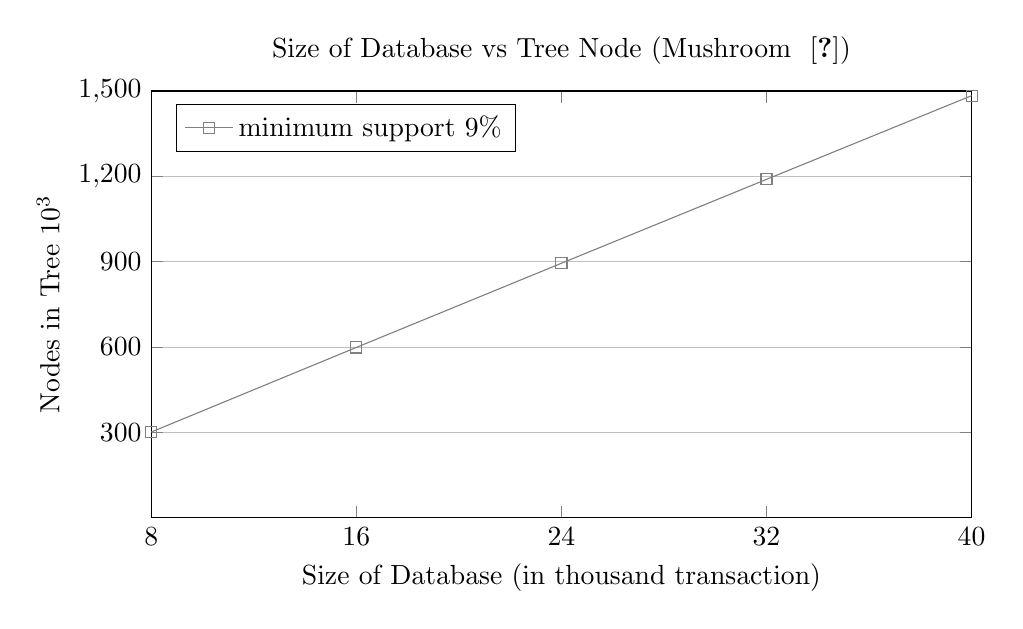
\begin{tikzpicture}
\begin{axis}[
	title={Size of Database vs Tree Node (Mushroom ~\cite{dataset})},
	width=12cm,
	height=7cm,
    xlabel={Size of Database (in thousand transaction)},
    ylabel={Nodes in Tree $10^3$},
    xmin=8, xmax=40,
    ymin=0, ymax=1500,
    xtick={8,16,24,32,40},
    ytick={300,600,900,1200,1500},
    legend pos=north west,
    ymajorgrids=true,
    grid style={line width=.2pt,draw=gray!50},
]
 
\addplot[
    solid,color=gray, every mark/.append style={solid, fill=gray}, mark=square
    ]
    coordinates {
			(8,300.856)
			(16,598.221)
			(24,894.225)
			(32,1189.166)
			(40,1483.378)



	};
    \addlegendentry{minimum support 9\%}

\end{axis}
\end{tikzpicture}
%\end{document}